\section{基本定义}

\subsection{精度误差}
\begin{frame}
计算几何题一个普遍的问题就是有精度误差。因为一般都设计到实数的加减乘除甚至开方、指数、对数，三角函数。所以我们通常需要设置一个精度误差范围eps。那么，判断两个数相等不再是$a=b$，而是$fabs(a-b)<eps$

\end{frame}

\subsection{向量}
\begin{frame}
为了运算的方便，我们一般把一个点或一个向量都用一个结构体存起来。在n维空间下向量的表示为$(a_1,a_2,\ldots,a_n)$。常用的就是二维向量，二维以上的用得较少。
\end{frame}

\begin{frame}
\frametitle{点积/数量积}
两个向量A,B的点积定义为$\sum_{i=1}^{n}a_i*b_i$，得到的是一个数。

同时$A \cdot B=|A||B|\cos(A,B)$
\end{frame}

\begin{frame}{叉积}
叉积是计算几何目前非常方便使用的工具。对于二维向量$A(x_1,y_1 ),B(x_2,y_2)$，它们的叉积$x_1*y_2-y_1*x_2$。叉积的含义是两个向量所夹的平行四边形的面积(/2后就是三角形面积)。

\pause
并且注意这里的面积是\textbf{有向}面积，方向遵循右手螺旋定则。伸出右手，将四指沿A沿小于平角旋转到B，如果选择时拇指朝上即为正方向，否则为负。
\end{frame}

\begin{frame}
\frametitle{向量的旋转}
向量$V(x,y)$逆时针旋转角度$\theta$后得到的向量可以直接用$x,y$及关于$\theta$的三角函数表示出来。(默认是逆时针)

\pause
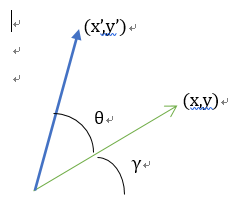
\includegraphics[width=3cm]{geometry/move.png}

\pause
\begin{displaymath}
|V|\cos(\theta + \gamma)=x' \ \ |V|\cos(\gamma)=x
\end{displaymath}

\begin{displaymath}
x'=\frac{ x \cos(\theta + \gamma) }{ \cos(\gamma) }=\frac{ x(\cos(\theta)\cos(\gamma) - \sin(\theta)\sin(\gamma) ) }{ \cos(\gamma) }
\end{displaymath}

\end{frame}

\begin{frame}

\pause
\begin{displaymath}
=x\cos(\theta)-x\sin(\theta)\tan(\gamma)=x\cos(\theta)-\sin(\theta)y
\end{displaymath}

\pause
同理可以求得$y'=x\sin(\theta)+y\cos(\theta)$

\pause
所以$rot((x,y),\theta)=(x\cos(\theta)-y\sin(\theta),x\sin(\theta)+y\cos(\theta))$

\pause
同时我们注意到向量的旋转是可以用矩阵乘法表示的
\begin{displaymath}
    [x \ y]*
    \left[
        \begin{array}{c @{\ } c}
            \cos(\theta)  & \sin(\theta) \\
            -\sin(\theta) & \cos(\theta)
        \end{array}
    \right]
\end{displaymath}
\end{frame}

\begin{frame}
\frametitle{向量的夹角}
求向量$\overrightarrow{a}$和向量$\overrightarrow{b}$的夹角

\begin{block}{方法一：}
$atan2(y_a,x_a)-atan2(y_b,x_b)$
\end{block}

\begin{block}{方法二：}
\begin{multicols}{2}
$atan2(\overrightarrow{a} \times \overrightarrow{b},\overrightarrow{a} \cdot \overrightarrow{b})$

解释：

$\overrightarrow{a} \times \overrightarrow{b}=|CD|*|AB|$

$\overrightarrow{a} \cdot \overrightarrow{b}=|AD| * |AB|$

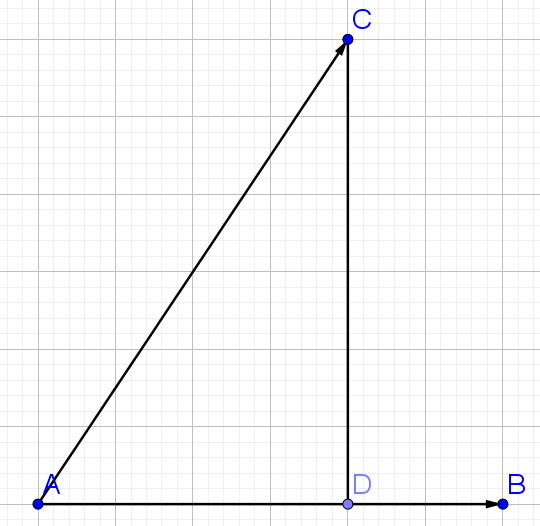
\includegraphics[height=2.5cm,width=3cm]{geometry/vector.png}
\end{multicols}
\end{block}

\pause
采用方法二更加好，因为方法一还要特判跨越了$\pi$到$-\pi$的情况，方法二不需要任何特判。
\end{frame}

\subsection{极角}

\begin{frame}
我们一般以x轴正方向为0刻度，从x轴正方向开始逆时针为正，顺时针为负。以x轴负方向为分界线。

特别地，x轴负方向的极角为$\pi$
\end{frame}

\subsection{重心}

\begin{frame}{三角形的重心}

三角形的重心是三条中线的交点。同时，重心把每条中线按照$1:2$的比例分割。

\pause
\begin{center}
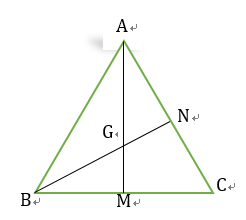
\includegraphics[width=3cm]{geometry/triangle.png}
\end{center}

\pause
\begin{displaymath}
M=\frac{B+C}{2}
\end{displaymath}
\begin{displaymath}
G=\frac{2}{3}M+\frac{1}{3}A=\frac{A+B+C}{3}
\end{displaymath}
\end{frame}

\begin{frame}{多边形的重心}

有一个定理：n个坐标为P，质量为M的质点的重心为

\begin{displaymath}
\sum_{i=1}^{n} P_i * \frac{M_i}{\sum_M}
\end{displaymath}

\pause
我们可以先把多边形进行三角剖分，然后得到所有三角形的重心，再以面积为权值计算加权平均数就是多边形的重心。
\end{frame}

\subsection{外心}
\begin{frame}

外心是指三角形外界圆的圆心

\pause
$\triangle ABC$解方程法

\begin{equation}
    (x-x_A)^2+(y-y_A)^2=(x-x_B)^2+(y-y_B)^2
\end{equation}
\begin{equation}
    (x-x_A)^2+(y-y_A)^2=(x-x_C)^2+(y-y_C)^2
\end{equation}

\pause
设
\begin{displaymath}
    A1=2(x_A-x_B),A2=2(x_A-x_C)
\end{displaymath}

\begin{displaymath}
    B1=2(y_A-y_B),B2=2(y_A-y_C)
\end{displaymath}

\begin{displaymath}
    C1=x_A^2+y_A^2-x_B^2-y_B^2,C2=x_A^2+y_A^2-x_C^2-y_C^2
\end{displaymath}
\end{frame}

\begin{frame}
\pause
\begin{equation}
    A1x+B1y=C1
\end{equation}
\begin{equation}
    A2x+B2y=C2
\end{equation}

\pause
根据克莱默法则
\begin{equation}
    x=\frac{ (C1*B2)-(C2*B1) }{ (A1*B2)-(A2*B1) }
\end{equation}
\begin{equation}
    y=\frac{ (A1*C2)-(A2*C1) }{ (A1*B2)-(A2*B1) }
\end{equation}
\end{frame}

\begin{frame}{几何法}

    也可以用几何法球外心

    外心就是三角形三条边垂直平分线的交点

    求出垂直平分线以后变成直线求交问题
\end{frame}

\subsection{内心}
\begin{frame}

三角形的内心为内切圆的圆心。\newline \newline

\href{https://en.wikipedia.org/wiki/Incenter}{\textcolor{purple}{维基}}上说三角形内切圆的圆心是三角形三个顶点A,B,C关于对边长度a,b,c的加权平均数，即
\begin{displaymath}
    inCenter=\frac{A*a+B*b+C*c}{a+b+c}
\end{displaymath}

（证明我不太懂，感兴趣的可以自行查阅）
\end{frame}
